\documentclass[a4paper,12pt]{article}

\usepackage[T2A]{fontenc}
\usepackage[utf8]{inputenc}
\usepackage[russian]{babel}
\usepackage{cmap}

\usepackage{amsmath,amssymb,mathtools}
\usepackage[a4paper,left=25mm,right=15mm,top=20mm,bottom=20mm]{geometry}
\usepackage{indentfirst}
\usepackage{graphicx}
\usepackage{float}
\usepackage{caption}
\usepackage{booktabs}
\usepackage{array}
\usepackage{tabularx}
\usepackage{enumitem}
\usepackage{titlesec}
\usepackage[unicode,hidelinks]{hyperref}

\captionsetup{labelsep=endash,font=small,skip=4pt}
\addto\captionsrussian{\renewcommand{\figurename}{Рисунок}}

\titleformat{\section}{\normalfont\large\bfseries}{\thesection}{0.6em}{}
\titleformat{\subsection}{\normalfont\normalsize\bfseries}{\thesubsection}{0.6em}{}
\titlespacing*{\section}{0pt}{14pt}{6pt}
\titlespacing*{\subsection}{0pt}{10pt}{4pt}

\setlength{\parindent}{1.25cm}
\setlength{\emergencystretch}{1.5em}
\linespread{1.1}
\setlist{itemsep=1pt,topsep=3pt}

\DeclareMathOperator{\diag}{diag}
\DeclareMathOperator{\sgn}{sign}
\renewcommand{\Re}{\operatorname{Re}}
\renewcommand{\Im}{\operatorname{Im}}

\begin{document}

\begin{center}
  {\Large\bfseries Классификация ДУЧП второго порядка\\[2pt]
   и приведение к каноническому виду\par}
  \vspace{6pt}
  {Отчёт по заданиям A, B, C\par}
  \vspace{4pt}
  {Выполнили: \rule{8cm}{0.4pt}\par}
\end{center}

\section*{Постановка задачи}

\begin{enumerate}[label=\textbf{\Alph*.}]
  \item Реализовать функцию, которая по коэффициентам ДУЧП второго порядка
        определяет его тип и замену переменных, приводящую уравнение
        к каноническому виду.
  \item Реализовать интерактивный виджет, который в реальном времени позволяет
        менять коэффициенты и показывает тип уравнения и замену переменных.
  \item Расширить классификатор на уравнения с переменными коэффициентами
        и определять области, в которых уравнение сохраняет свой тип.
\end{enumerate}

Встроенные функции, выполняющие эти задачи, не использовались.

% ======================================================================
\section{Теоретические сведения}

\subsection{Канонический вид уравнения с \texorpdfstring{$n$}{n} независимыми переменными}
\label{ss:n}

Рассматривается уравнение, линейное относительно старших производных:
\begin{equation}\label{eq:general}
  \sum_{i=1}^{n}\sum_{j=1}^{n} a_{ij}\,u_{x_i x_j}
  + F\bigl(x_1,\dots,x_n,u,u_{x_1},\dots,u_{x_n}\bigr) = 0,
  \qquad a_{ij}=a_{ji}.
\end{equation}
Ему соответствует характеристическая квадратичная форма
\begin{equation}\label{eq:Q}
  Q(\lambda_1,\dots,\lambda_n)=\sum_{i=1}^{n}\sum_{j=1}^{n} a_{ij}\lambda_i\lambda_j
  =\lambda^{\mathsf T}\!A\lambda,
  \qquad A=\bigl(a_{ij}\bigr).
\end{equation}
Невырожденным линейным преобразованием $\lambda=P\mu$ форма~\eqref{eq:Q}
приводится к каноническому виду
\begin{equation}\label{eq:Qcan}
  Q=\sum_{i=1}^{n}\beta_i\mu_i^{2},
  \qquad P^{\mathsf T}\!AP=\diag(\beta_1,\dots,\beta_n).
\end{equation}

Пусть в уравнении~\eqref{eq:general} выполнена линейная замена $\xi=Mx$,
$u(x)=v(\xi)$. Тогда
\[
  u_{x_i}=\sum_{k=1}^{n}M_{ki}\,v_{\xi_k},\qquad
  u_{x_ix_j}=\sum_{k=1}^{n}\sum_{l=1}^{n}M_{ki}M_{lj}\,v_{\xi_k\xi_l},
\]
и старшая часть уравнения преобразуется по правилу
\[
  \sum_{i,j}a_{ij}\,u_{x_ix_j}=\sum_{k,l}\bigl(MAM^{\mathsf T}\bigr)_{kl}\,v_{\xi_k\xi_l}.
\]
При $M=P^{\mathsf T}$ выполняется $MAM^{\mathsf T}=P^{\mathsf T}\!AP=\diag(\beta)$,
поэтому замена
\begin{equation}\label{eq:subst}
  \xi=P^{\mathsf T}x
\end{equation}
приводит уравнение~\eqref{eq:general} к каноническому виду
\begin{equation}\label{eq:can}
  \sum_{i=1}^{n}\beta_i\,v_{\xi_i\xi_i}
  +\tilde F\bigl(\xi,v,v_{\xi_1},\dots,v_{\xi_n}\bigr)=0.
\end{equation}
Младшие члены при линейной замене преобразуются по правилу
$\sum_i b_i\,u_{x_i}=\sum_k (Mb)_k\,v_{\xi_k}$.

Тип уравнения определяется набором коэффициентов $\beta_i$:
\begin{itemize}
  \item гиперболический --- все $\beta_i\neq0$ и не все одного знака;
  \item параболический --- среди $\beta_i$ есть нулевые, а ненулевые одного знака;
  \item эллиптический --- все $\beta_i\neq0$ и все одного знака.
\end{itemize}

\subsection{Случай двух независимых переменных}
\label{ss:2d}

Уравнение с двумя независимыми переменными имеет вид
\begin{equation}\label{eq:2d}
  a_{11}u_{xx}+2a_{12}u_{xy}+a_{22}u_{yy}+F(x,y,u,u_x,u_y)=0.
\end{equation}
При замене $\xi=\xi(x,y)$, $\eta=\eta(x,y)$ производные пересчитываются по формулам
\begin{align*}
  u_x    &= u_\xi\xi_x+u_\eta\eta_x, \qquad u_y = u_\xi\xi_y+u_\eta\eta_y,\\
  u_{xx} &= u_{\xi\xi}\xi_x^2+2u_{\xi\eta}\xi_x\eta_x+u_{\eta\eta}\eta_x^2
            +u_\xi\xi_{xx}+u_\eta\eta_{xx},\\
  u_{xy} &= u_{\xi\xi}\xi_x\xi_y+u_{\xi\eta}(\xi_x\eta_y+\xi_y\eta_x)
            +u_{\eta\eta}\eta_x\eta_y+u_\xi\xi_{xy}+u_\eta\eta_{xy},\\
  u_{yy} &= u_{\xi\xi}\xi_y^2+2u_{\xi\eta}\xi_y\eta_y+u_{\eta\eta}\eta_y^2
            +u_\xi\xi_{yy}+u_\eta\eta_{yy}.
\end{align*}
В новых переменных уравнение~\eqref{eq:2d} принимает вид
\begin{equation}\label{eq:2dnew}
  \bar a_{11}u_{\xi\xi}+2\bar a_{12}u_{\xi\eta}+\bar a_{22}u_{\eta\eta}+\bar F=0,
\end{equation}
где
\begin{equation}\label{eq:abar}
\begin{aligned}
  \bar a_{11}&=a_{11}\xi_x^2+2a_{12}\xi_x\xi_y+a_{22}\xi_y^2,\\
  \bar a_{12}&=a_{11}\xi_x\eta_x+a_{12}(\xi_x\eta_y+\xi_y\eta_x)+a_{22}\xi_y\eta_y,\\
  \bar a_{22}&=a_{11}\eta_x^2+2a_{12}\eta_x\eta_y+a_{22}\eta_y^2.
\end{aligned}
\end{equation}
Если уравнение содержит младшие члены $b_1u_x+b_2u_y+cu$, то коэффициенты при
$u_\xi$ и $u_\eta$ равны
\begin{equation}\label{eq:bbar}
\begin{aligned}
  \bar b_1&=a_{11}\xi_{xx}+2a_{12}\xi_{xy}+a_{22}\xi_{yy}+b_1\xi_x+b_2\xi_y,\\
  \bar b_2&=a_{11}\eta_{xx}+2a_{12}\eta_{xy}+a_{22}\eta_{yy}+b_1\eta_x+b_2\eta_y.
\end{aligned}
\end{equation}

Коэффициент $\bar a_{11}$ обращается в нуль, если $\xi(x,y)=C$ --- общий интеграл
характеристического уравнения
\begin{equation}\label{eq:char}
  a_{11}\,dy^2-2a_{12}\,dx\,dy+a_{22}\,dx^2=0.
\end{equation}
Его дискриминант
\begin{equation}\label{eq:D}
  D=a_{12}^2-a_{11}a_{22}
   =-\begin{vmatrix}a_{11}&a_{12}\\ a_{12}&a_{22}\end{vmatrix},
\end{equation}
и при $a_{11}\neq0$ уравнение~\eqref{eq:char} распадается на два:
\begin{equation}\label{eq:roots}
  \frac{dy}{dx}=\frac{a_{12}\pm\sqrt{D}}{a_{11}}.
\end{equation}

\begin{itemize}
  \item $D>0$ --- гиперболический тип. Существуют две действительные характеристики
        $\varphi(x,y)=C_1$, $\psi(x,y)=C_2$. Замена $\xi=\varphi$, $\eta=\psi$ даёт
        $\bar a_{11}=\bar a_{22}=0$ и первую каноническую форму $u_{\xi\eta}=\Phi$.
        Заменой $\sigma=\xi+\eta$, $\tau=\xi-\eta$ она переводится во вторую:
        $u_{\sigma\sigma}-u_{\tau\tau}=\Phi_1$.
  \item $D=0$ --- параболический тип. Существует одна характеристика
        $\varphi(x,y)=C$. Полагается $\xi=\varphi$, а $\eta$ выбирается произвольно
        при условии
        $J=\begin{vmatrix}\xi_x&\xi_y\\ \eta_x&\eta_y\end{vmatrix}\neq0$.
        Получается $\bar a_{11}=\bar a_{12}=0$ и канонический вид
        $u_{\eta\eta}=\Phi$.
  \item $D<0$ --- эллиптический тип. Корни комплексно сопряжены,
        $\varphi(x,y)\pm i\psi(x,y)=C$. Замена $\xi=\varphi$, $\eta=\psi$ даёт
        $\bar a_{12}=0$, $\bar a_{11}=\bar a_{22}$ и канонический вид
        $u_{\xi\xi}+u_{\eta\eta}=\Phi$.
\end{itemize}

\subsection{Уравнения с переменными коэффициентами}

Если коэффициенты $a_{11},a_{12},a_{22}$ зависят от $x$ и $y$, то дискриминант
$D(x,y)=a_{12}^2-a_{11}a_{22}$ является функцией точки. Тип уравнения в точке
определяется знаком $D$, и плоскость разбивается на множества
\[
  \Omega_{+}=\{D>0\},\qquad \Omega_{0}=\{D=0\},\qquad \Omega_{-}=\{D<0\},
\]
в которых уравнение соответственно гиперболическое, параболическое и
эллиптическое. Приведение к каноническому виду выполняется в каждой области
отдельно.

% ======================================================================
\section{Задание A. Определение типа и замены переменных}

\subsection{Реализация}

Программа написана на языке Python~3. Библиотека \texttt{sympy} использована для
точной арифметики (рациональные числа, радикалы), дифференцирования и
интегрирования, библиотека \texttt{matplotlib} --- для построения графиков.
Алгоритмы классификации и приведения реализованы в пакете
\texttt{pde\_canonical}:
\begin{itemize}
  \item \texttt{exact.py} --- умножение и транспонирование матриц, обращение матрицы
        методом Гаусса--Жордана;
  \item \texttt{lagrange.py} --- приведение квадратичной формы к сумме квадратов
        методом Лагранжа;
  \item \texttt{classifier.py} --- тип уравнения и замена $\xi=P^{\mathsf T}x$
        для $n$ переменных;
  \item \texttt{characteristics.py} --- метод характеристик для двух переменных;
  \item \texttt{regions.py} --- области сохранения типа (задание C).
\end{itemize}
Кроме того, в проект входят: \texttt{demo.py} --- расчёт примеров,
\texttt{plot\_regions.py} --- построение карт областей,
\texttt{widget/index.html} --- виджет (задание B), каталог \texttt{tests} ---
автоматические тесты.

\subsection{Алгоритм для \texorpdfstring{$n$}{n} переменных (метод Лагранжа)}

На вход подаётся симметричная матрица $A=(a_{ij})$. Текущая форма хранится
матрицей $B$ (в начале $B=A$), множество необработанных индексов --- $K$
(в начале $K=\{1,\dots,n\}$).

\textbf{Шаг 1.} Если существует $k\in K$, для которого $b_{kk}\neq0$, выделяется
полный квадрат:
\begin{equation}\label{eq:square}
  Q=b_{kk}\Bigl(\lambda_k+\sum_{j\in K,\,j\neq k}\frac{b_{kj}}{b_{kk}}\lambda_j\Bigr)^{2}+Q',
\end{equation}
где $Q'$ --- форма от оставшихся переменных с коэффициентами
\begin{equation}\label{eq:schur}
  b'_{ij}=b_{ij}-\frac{b_{ki}\,b_{kj}}{b_{kk}},\qquad i,j\in K\setminus\{k\}.
\end{equation}
Полагается
\[
  \mu_k=\sqrt{|b_{kk}|}\,\Bigl(\lambda_k+\sum_{j\in K,\,j\neq k}\frac{b_{kj}}{b_{kk}}\lambda_j\Bigr),
  \qquad \beta_k=\sgn b_{kk},
\]
и индекс $k$ исключается из $K$.

\textbf{Шаг 2.} Если все $b_{kk}=0$ ($k\in K$), но есть $b_{ij}\neq0$, выполняется
замена
\begin{equation}\label{eq:pair}
  \lambda_i=\frac{\nu_i+\nu_j}{2},\qquad \lambda_j=\frac{\nu_i-\nu_j}{2},
  \qquad \lambda_i\lambda_j=\frac{\nu_i^2-\nu_j^2}{4},
\end{equation}
после которой в форме появляются квадраты, и выполняется шаг~1. В матричном виде
$B\to S^{\mathsf T}BS$, где $S$ --- матрица замены~\eqref{eq:pair}.

\textbf{Шаг 3.} Если все коэффициенты оставшейся части формы равны нулю, то для
$k\in K$ полагается $\beta_k=0$, а $\mu_k$ совпадает с текущей переменной
с номером $k$.

По построению $\mu=C\lambda$, где строки матрицы $C$ --- коэффициенты выражений
$\mu_k$ через исходные переменные $\lambda$. Далее вычисляются $P=C^{-1}$ методом
Гаусса--Жордана и замена $\xi=P^{\mathsf T}x$. Правильность приведения проверяется
тождеством $P^{\mathsf T}\!AP=\diag(\beta)$. Тип определяется по знакам $\beta_i$
(п.~\ref{ss:n}). Дополнительно отмечаются ультрагиперболический случай ($n\ge4$,
положительных и отрицательных $\beta_i$ не меньше двух) и ультрапараболический
(есть нулевые $\beta_i$, а ненулевые разных знаков).

\subsection{Алгоритм для двух переменных (метод характеристик)}

\begin{enumerate}
  \item Вычисляется $D=a_{12}^2-a_{11}a_{22}$ и по его знаку определяется тип.
  \item Находятся корни характеристического уравнения. При $a_{11}\neq0$
        используется формула~\eqref{eq:roots}. При $a_{11}=0$, $a_{22}\neq0$
        уравнение~\eqref{eq:char} решается относительно $dx/dy$:
        \[
          a_{22}\Bigl(\frac{dx}{dy}\Bigr)^2-2a_{12}\frac{dx}{dy}+a_{11}=0,
          \qquad
          \frac{dx}{dy}=\frac{a_{12}\pm\sqrt{D}}{a_{22}}.
        \]
        При $a_{11}=a_{22}=0$ уравнение~\eqref{eq:char} имеет вид $dx\,dy=0$,
        характеристики $x=C_1$, $y=C_2$.
  \item Интегрируется уравнение $dy/dx=\lambda(x,y)$. Если $\lambda$ не зависит
        от $y$, то $\varphi=y-\int\lambda\,dx$; если $\lambda$ не зависит от $x$, то
        $\varphi=\int\frac{dy}{\lambda}-x$; если $\lambda=f(x)\,g(y)$, то
        $\varphi=\int\frac{dy}{g(y)}-\int f(x)\,dx$.
  \item Новые переменные выбираются по правилам п.~\ref{ss:2d}; для
        эллиптического типа $\xi=\Re\varphi$, $\eta=\Im\varphi$.
  \item Выполняется проверка: вычисляются якобиан $J=\xi_x\eta_y-\xi_y\eta_x$ и
        коэффициенты~\eqref{eq:abar}. Должно выполняться $J\neq0$, а также
        $\bar a_{11}=\bar a_{22}=0$ для гиперболического типа,
        $\bar a_{11}=\bar a_{12}=0$ для параболического,
        $\bar a_{12}=0$, $\bar a_{11}=\bar a_{22}$ для эллиптического.
\end{enumerate}

\subsection{Результаты}

\paragraph{Пример 1.} $u_{xy}-2u_{xz}+u_{yz}+u_x+\tfrac12u_y=0$.

Матрица формы и сама форма:
\[
  A=\begin{pmatrix}0&\tfrac12&-1\\[2pt]\tfrac12&0&\tfrac12\\[2pt]-1&\tfrac12&0\end{pmatrix},
  \qquad
  Q=\lambda_1\lambda_2-2\lambda_1\lambda_3+\lambda_2\lambda_3.
\]
Квадратов нет, поэтому сначала выполняется замена~\eqref{eq:pair} при $i=1$, $j=2$:
\[
  Q=\tfrac14\nu_1^2-\tfrac14\nu_2^2-\tfrac12\nu_1\nu_3-\tfrac32\nu_2\nu_3
   =\Bigl\{\tfrac12(\nu_1-\nu_3)\Bigr\}^2-\Bigl\{\tfrac12(\nu_2+3\nu_3)\Bigr\}^2
    +\bigl\{\sqrt2\,\nu_3\bigr\}^2.
\]
С учётом $\nu_1=\lambda_1+\lambda_2$, $\nu_2=\lambda_1-\lambda_2$, $\nu_3=\lambda_3$:
\[
  \beta=(1,-1,1),\qquad
  C=\begin{pmatrix}\tfrac12&\tfrac12&-\tfrac12\\[2pt]\tfrac12&-\tfrac12&\tfrac32\\[2pt]0&0&\sqrt2\end{pmatrix},
  \qquad
  P=C^{-1}=\begin{pmatrix}1&1&-\tfrac{\sqrt2}{2}\\[2pt]1&-1&\sqrt2\\[2pt]0&0&\tfrac{\sqrt2}{2}\end{pmatrix}.
\]
Все $\beta_i\neq0$ и разных знаков, уравнение гиперболическое.
Замена $\xi=P^{\mathsf T}x$:
\[
  \xi=x+y,\qquad \eta=x-y,\qquad
  \omega=-\tfrac{\sqrt2}{2}\,x+\sqrt2\,y+\tfrac{\sqrt2}{2}\,z.
\]
Проверка: $P^{\mathsf T}\!AP=\diag(1,-1,1)$. Младшие члены: $b=(1,\tfrac12,0)^{\mathsf T}$,
$P^{\mathsf T}b=(\tfrac32,\tfrac12,0)^{\mathsf T}$. Канонический вид:
\[
  v_{\xi\xi}-v_{\eta\eta}+v_{\omega\omega}+\tfrac32\,v_\xi+\tfrac12\,v_\eta=0.
\]

\paragraph{Пример 2.} $u_{xx}+2u_{xy}+5u_{yy}-32u=0$.
\begin{gather*}
  Q=\lambda_1^2+2\lambda_1\lambda_2+5\lambda_2^2=(\lambda_1+\lambda_2)^2+(2\lambda_2)^2,\\
  \beta=(1,1),\qquad
  C=\begin{pmatrix}1&1\\0&2\end{pmatrix},\qquad
  P=\begin{pmatrix}1&-\tfrac12\\[2pt]0&\tfrac12\end{pmatrix}.
\end{gather*}
Уравнение эллиптическое. Замена $\xi=x$, $\eta=-\tfrac12x+\tfrac12y$,
канонический вид:
\[
  v_{\xi\xi}+v_{\eta\eta}-32v=0.
\]

\paragraph{Пример 3.} $u_{xx}-2u_{xy}+u_{yy}+9u_x+9u_y-9u=0$.

Здесь $a_{11}=1$, $a_{12}=-1$, $a_{22}=1$, $D=1-1=0$, уравнение параболическое.
Характеристическое уравнение
$\bigl(\frac{dy}{dx}\bigr)^2+2\frac{dy}{dx}+1=0$ имеет корень $\frac{dy}{dx}=-1$,
характеристика $x+y=C$. Замена $\xi=x+y$, $\eta=x$, якобиан $J=-1$.
По формулам~\eqref{eq:abar} и~\eqref{eq:bbar}:
\[
  \bar a_{11}=0,\quad \bar a_{12}=0,\quad \bar a_{22}=1,\qquad
  \bar b_1=9\xi_x+9\xi_y=18,\quad \bar b_2=9\eta_x+9\eta_y=9.
\]
Канонический вид:
\[
  v_{\eta\eta}+18v_\xi+9v_\eta-9v=0.
\]

Результаты приведения классических уравнений методом характеристик приведены
в таблице~\ref{tab:classic}.

\begin{table}[H]
\centering\small
\renewcommand{\arraystretch}{1.3}
\setlength{\tabcolsep}{4pt}
\caption{Приведение классических уравнений}
\label{tab:classic}
\begin{tabular}{@{}lccccc@{}}
\toprule
Уравнение & $D$ & Тип & Замена & $(\bar a_{11},\bar a_{12},\bar a_{22})$ & Канонический вид\\
\midrule
$u_{xx}-u_{yy}=0$ & $1$  & гиперболический & $\xi=y-x,\ \eta=y+x$ & $(0,-2,0)$ & $u_{\xi\eta}=0$\\
$u_{xx}-u_{y}=0$  & $0$  & параболический  & $\xi=y,\ \eta=x$     & $(0,0,1)$  & $u_{\eta\eta}-u_\xi=0$\\
$u_{xx}+u_{yy}=0$ & $-1$ & эллиптический   & $\xi=y,\ \eta=x$     & $(1,0,1)$  & $u_{\xi\xi}+u_{\eta\eta}=0$\\
\bottomrule
\end{tabular}
\end{table}

% ======================================================================
\section{Задание B. Интерактивный виджет}

Виджет выполнен в виде одной HTML-страницы \texttt{widget/index.html} с кодом на
JavaScript. Все вычисления выполняются в браузере; подключение к сети и установка
дополнительного программного обеспечения не требуются.

Виджет имеет три режима.
\begin{enumerate}
  \item \textbf{Две переменные.} Коэффициенты $a_{11},a_{12},a_{22}$ задаются
        ползунками или числовыми полями. При каждом изменении пересчитываются
        дискриминант $D$, тип уравнения, характеристики, замена $\xi,\eta$,
        якобиан $J$, коэффициенты $\bar a_{11},\bar a_{12},\bar a_{22}$ и
        канонический вид; выводится ход решения (рисунок~\ref{fig:wconst}).
  \item \textbf{Переменные коэффициенты.} Коэффициенты вводятся как выражения от
        $x$ и $y$; допустимы числа, операции \verb|+ - * / ^|, скобки и функции
        \texttt{sqrt}, \texttt{sin}, \texttt{cos}, \texttt{exp}, \texttt{abs}.
        Строится карта областей по знаку $D(x,y)$. При наведении курсора выводятся
        значение $D$ и тип в точке, при щелчке --- разбор уравнения с коэффициентами,
        вычисленными в этой точке (рисунок~\ref{fig:wvar}).
  \item \textbf{$n$ переменных.} Задаётся матрица $(a_{ij})$ размера до $5\times5$.
        Выполняется метод Лагранжа, выводятся $\beta$, тип, замена
        $\xi=P^{\mathsf T}x$ и результат проверки $P^{\mathsf T}\!AP=\diag(\beta)$.
\end{enumerate}

В режиме $n$ переменных используется точная рациональная арифметика: числитель
и знаменатель дроби хранятся как целые числа произвольной длины (\texttt{BigInt}),
поэтому погрешности округления не возникают. Выражения $a_{ij}(x,y)$ разбираются
рекурсивным нисходящим анализатором. Карта областей строится вычислением знака $D$
в узлах сетки; граница $D=0$ отмечается там, где знак меняется у соседних узлов.
В каждом режиме предусмотрены готовые примеры: волновое уравнение, уравнение
теплопроводности, уравнение Лапласа, уравнение Трикоми и примеры из лекции.

\begin{figure}[!htbp]
\centering
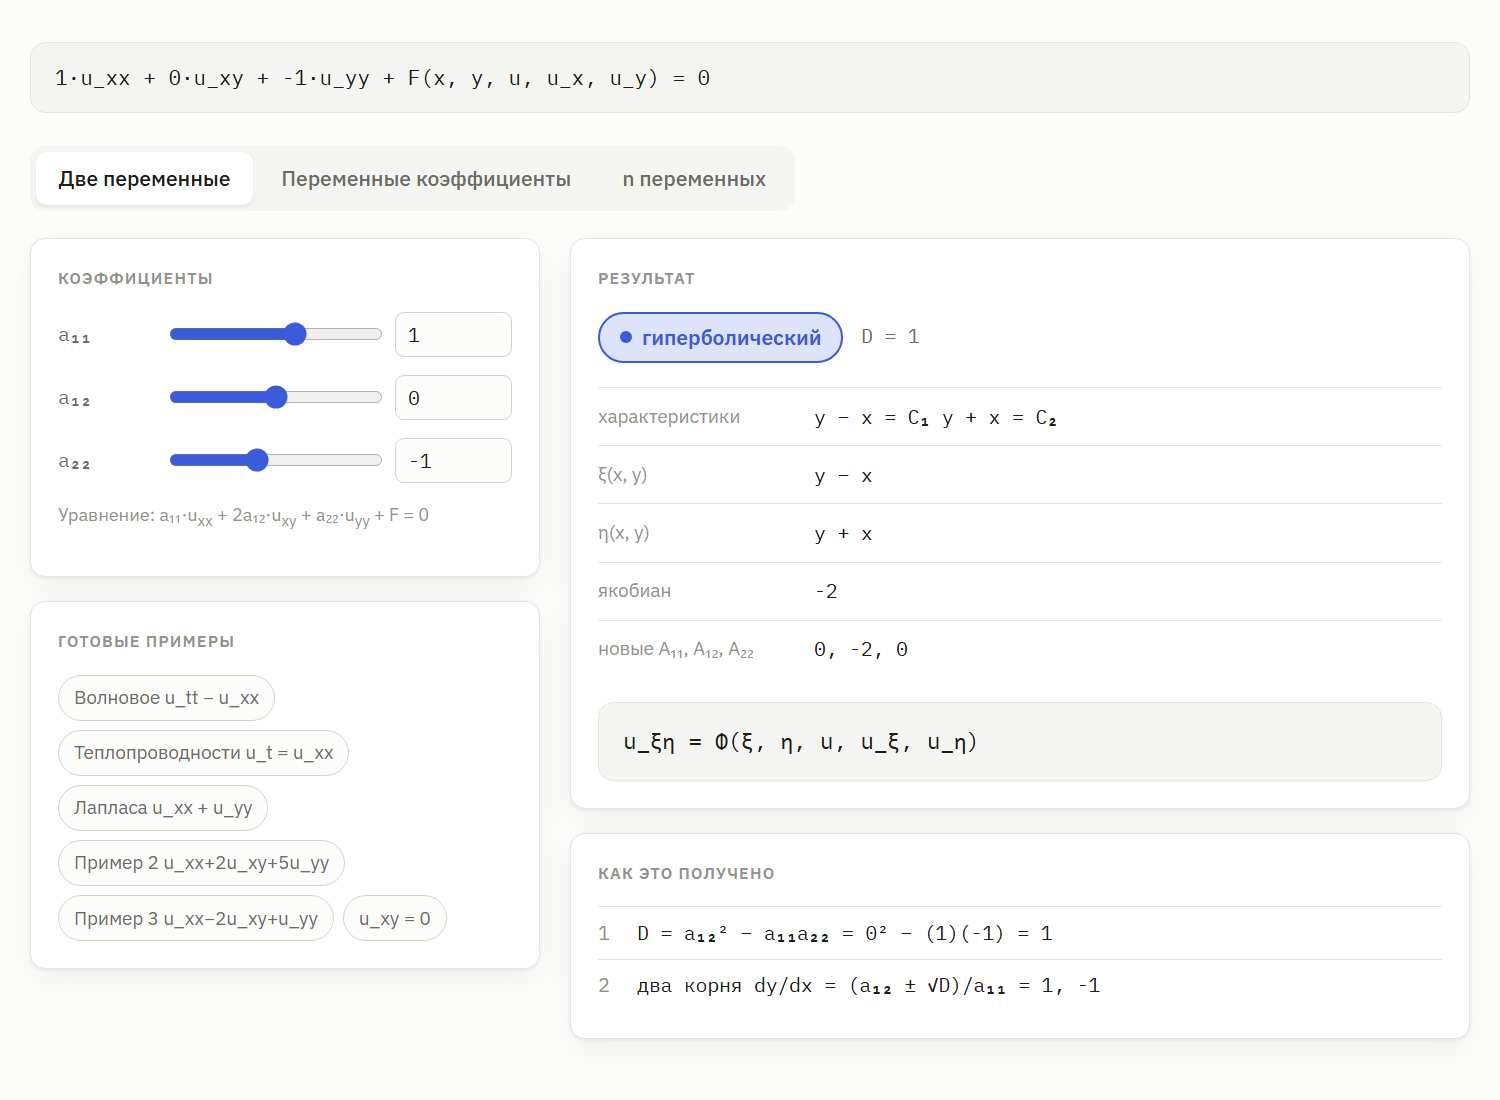
\includegraphics[width=\textwidth,height=0.5\textheight,keepaspectratio]{figures/widget_const.png}
\caption{Режим «Две переменные», волновое уравнение}
\label{fig:wconst}
\end{figure}

\begin{figure}[!htbp]
\centering
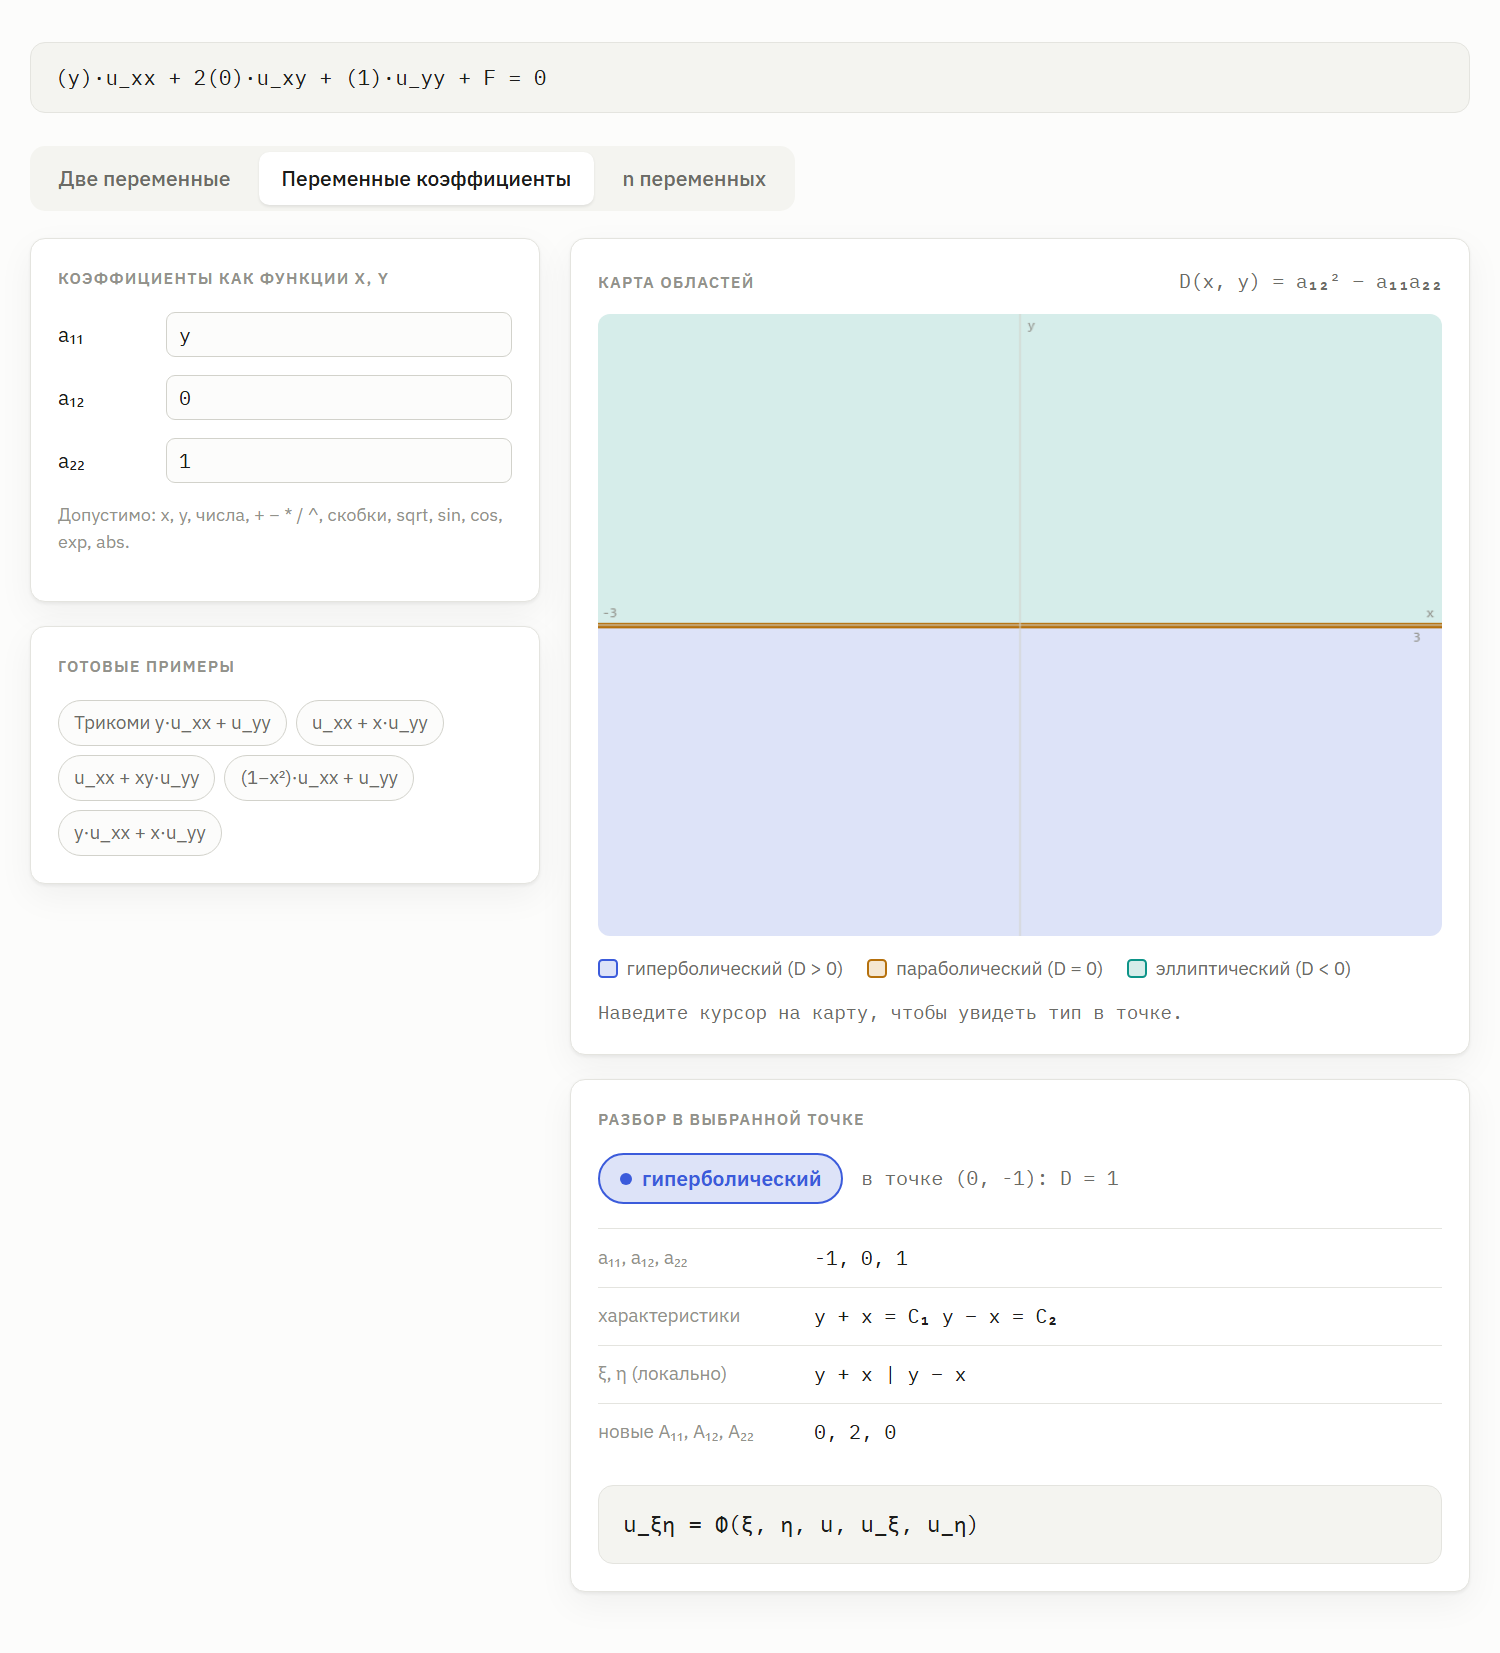
\includegraphics[width=\textwidth,height=0.6\textheight,keepaspectratio]{figures/widget_var.png}
\caption{Режим «Переменные коэффициенты», уравнение Трикоми}
\label{fig:wvar}
\end{figure}

% ======================================================================
\section{Задание C. Уравнения с переменными коэффициентами}

\subsection{Алгоритм}

\begin{enumerate}
  \item Символьно вычисляется $D(x,y)=a_{12}^2-a_{11}a_{22}$.
  \item Если $D$ не зависит от $x$ и $y$, уравнение имеет один тип во всей плоскости.
  \item Если $D$ зависит от одной переменной $t\in\{x,y\}$, находятся действительные
        корни $t_1<\dots<t_m$ уравнения $D=0$. Прямые $t=t_k$ разбивают плоскость на
        полосы $t<t_1$, $t_k<t<t_{k+1}$, $t>t_m$; тип в каждой полосе и на каждой
        границе определяется знаком $D$ в пробной точке.
  \item Если $D$ зависит от обеих переменных, знак $D$ вычисляется в узлах сетки,
        а области постоянного знака выделяются как связные компоненты.
  \item В каждой области уравнение приводится к каноническому виду методом
        характеристик с учётом знака переменной. При $y<0$ выполняется подстановка
        $y=-s$, $s>0$. Так как $dy=-ds$, характеристическое
        уравнение~\eqref{eq:char} принимает вид
        \begin{equation}\label{eq:charflip}
          a_{11}\,ds^2+2a_{12}\,dx\,ds+a_{22}\,dx^2=0,
        \end{equation}
        то есть коэффициент при $dx\,ds$ меняет знак. После интегрирования
        выполняется обратная подстановка $s=-y$.
\end{enumerate}

\subsection{Уравнение Трикоми}

Рассматривается уравнение
\begin{equation}\label{eq:tricomi}
  y\,u_{xx}+u_{yy}=0,\qquad a_{11}=y,\quad a_{12}=0,\quad a_{22}=1.
\end{equation}
Дискриминант $D=-y$, следовательно, при $y<0$ уравнение гиперболическое,
при $y=0$ --- параболическое, при $y>0$ --- эллиптическое
(рисунок~\ref{fig:tricomi}).
Характеристическое уравнение:
\[
  y\,dy^2+dx^2=0\quad\Longleftrightarrow\quad\Bigl(\frac{dy}{dx}\Bigr)^2=-\frac1y.
\]

\paragraph{Область $y<0$.}
$\dfrac{dy}{dx}=\pm\dfrac{1}{\sqrt{-y}}$, откуда $\sqrt{-y}\,dy=\pm dx$ и
\[
  x\pm\tfrac23(-y)^{3/2}=C.
\]
Замена:
\[
  \xi=x+\tfrac23(-y)^{3/2},\qquad \eta=x-\tfrac23(-y)^{3/2}.
\]
Производные:
\[
  \xi_x=\eta_x=1,\quad \xi_y=-\sqrt{-y},\quad \eta_y=\sqrt{-y},\quad
  \xi_{yy}=\frac{1}{2\sqrt{-y}},\quad \eta_{yy}=-\frac{1}{2\sqrt{-y}}.
\]
По формулам~\eqref{eq:abar} и~\eqref{eq:bbar}:
\[
  \bar a_{11}=0,\quad \bar a_{12}=2y,\quad \bar a_{22}=0,\qquad
  \bar b_1=\frac{1}{2\sqrt{-y}},\quad \bar b_2=-\frac{1}{2\sqrt{-y}},
\]
и уравнение принимает вид
\[
  4y\,u_{\xi\eta}+\frac{1}{2\sqrt{-y}}\,(u_\xi-u_\eta)=0.
\]
Так как $\xi-\eta=\tfrac43(-y)^{3/2}$, то $\dfrac{1}{8y\sqrt{-y}}=-\dfrac{1}{8(-y)^{3/2}}=-\dfrac{1}{6(\xi-\eta)}$,
и канонический вид
\[
  u_{\xi\eta}-\frac{1}{6(\xi-\eta)}\,(u_\xi-u_\eta)=0.
\]

\paragraph{Прямая $y=0$.} Уравнение вырождается в $u_{yy}=0$
($a_{11}=a_{12}=0$, $a_{22}=1$). Характеристика $x=C$; замена $\xi=x$, $\eta=y$
даёт канонический вид
\[
  u_{\eta\eta}=0.
\]

\paragraph{Область $y>0$.}
$\dfrac{dy}{dx}=\pm\dfrac{i}{\sqrt{y}}$, откуда $\sqrt{y}\,dy=\pm i\,dx$ и
\[
  \tfrac23\,y^{3/2}\mp i\,x=C.
\]
Замена:
\[
  \xi=x,\qquad \eta=\tfrac23\,y^{3/2}.
\]
Производные: $\xi_x=1$, $\xi_y=0$, $\eta_x=0$, $\eta_y=\sqrt{y}$,
$\eta_{yy}=\dfrac{1}{2\sqrt{y}}$. Тогда
\[
  \bar a_{11}=y,\quad \bar a_{12}=0,\quad \bar a_{22}=y,\qquad
  \bar b_1=0,\quad \bar b_2=\frac{1}{2\sqrt{y}},
\]
и уравнение принимает вид
\[
  y\,(u_{\xi\xi}+u_{\eta\eta})+\frac{1}{2\sqrt{y}}\,u_\eta=0.
\]
Так как $y^{3/2}=\tfrac32\eta$, канонический вид
\[
  u_{\xi\xi}+u_{\eta\eta}+\frac{1}{3\eta}\,u_\eta=0.
\]
Результаты по областям сведены в таблицу~\ref{tab:tricomi}.

\begin{table}[H]
\centering\small
\renewcommand{\arraystretch}{1.5}
\setlength{\tabcolsep}{4pt}
\caption{Уравнение Трикоми по областям}
\label{tab:tricomi}
\begin{tabular}{@{}cccc@{}}
\toprule
Область & Тип & Замена & Канонический вид\\
\midrule
$y<0$ & гиперболический & $\xi,\eta=x\pm\frac23(-y)^{3/2}$ & $u_{\xi\eta}-\frac{1}{6(\xi-\eta)}(u_\xi-u_\eta)=0$\\
$y=0$ & параболический  & $\xi=x,\ \eta=y$                 & $u_{\eta\eta}=0$\\
$y>0$ & эллиптический   & $\xi=x,\ \eta=\frac23y^{3/2}$    & $u_{\xi\xi}+u_{\eta\eta}+\frac{1}{3\eta}u_\eta=0$\\
\bottomrule
\end{tabular}
\end{table}

\begin{figure}[!htbp]
\centering
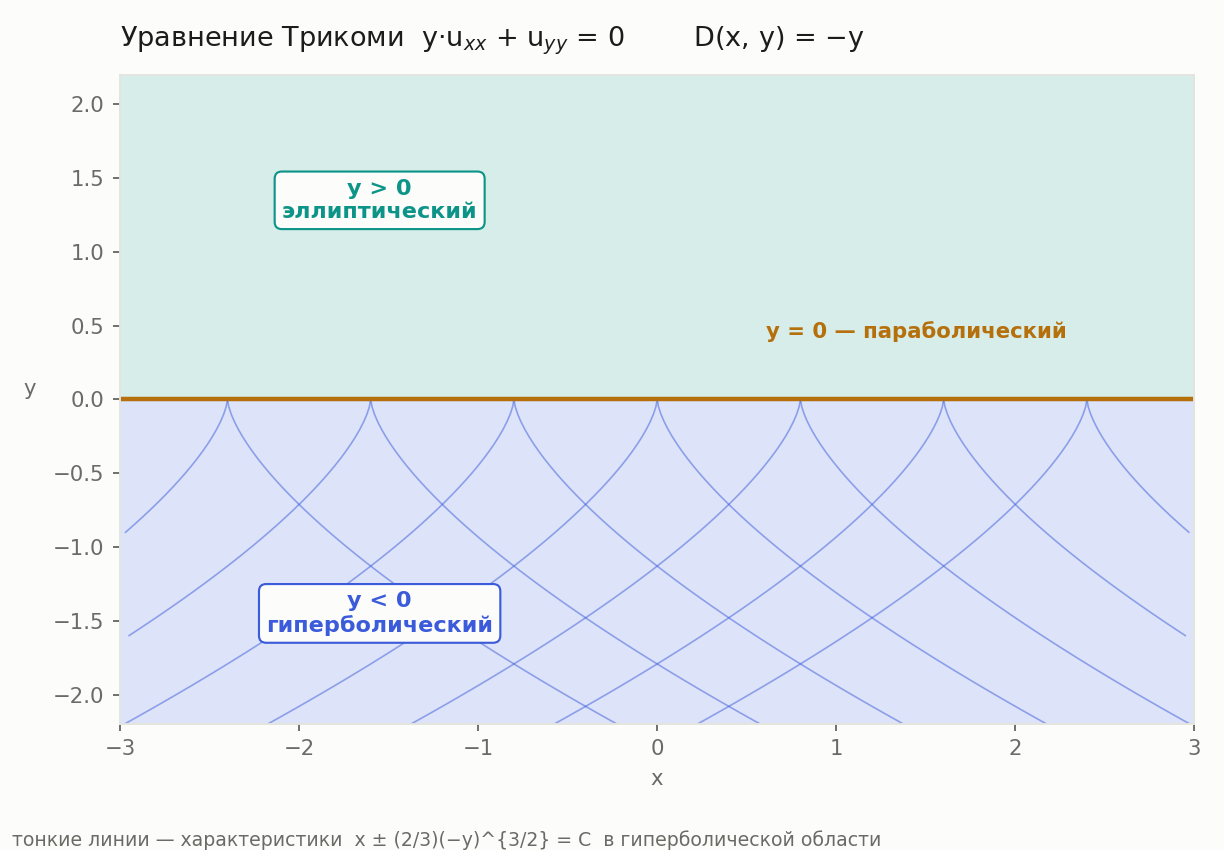
\includegraphics[width=0.88\textwidth]{figures/regions_tricomi.png}
\caption{Области сохранения типа для уравнения Трикоми; тонкие линии ---
характеристики $x\pm\frac23(-y)^{3/2}=C$}
\label{fig:tricomi}
\end{figure}

\subsection{Другие примеры}

Области сохранения типа для других уравнений с переменными коэффициентами
приведены в таблице~\ref{tab:regions} и на рисунке~\ref{fig:gallery}.

\begin{table}[H]
\centering\small
\renewcommand{\arraystretch}{1.35}
\caption{Области сохранения типа}
\label{tab:regions}
\begin{tabularx}{\textwidth}{@{}l c >{\raggedright\arraybackslash}X@{}}
\toprule
Уравнение & $D(x,y)$ & Области и тип\\
\midrule
$u_{xx}+x\,u_{yy}=0$ & $-x$ &
  $x<0$ --- гиперболический; $x=0$ --- параболический; $x>0$ --- эллиптический\\
$u_{xx}+xy\,u_{yy}=0$ & $-xy$ &
  $xy<0$ (II и IV четверти) --- гиперболический; $xy=0$ --- параболический;
  $xy>0$ (I и III четверти) --- эллиптический\\
$(1-x^2)\,u_{xx}+u_{yy}=0$ & $x^2-1$ &
  $|x|>1$ --- гиперболический; $x=\pm1$ --- параболический; $|x|<1$ --- эллиптический\\
\bottomrule
\end{tabularx}
\end{table}

\begin{figure}[!htbp]
\centering
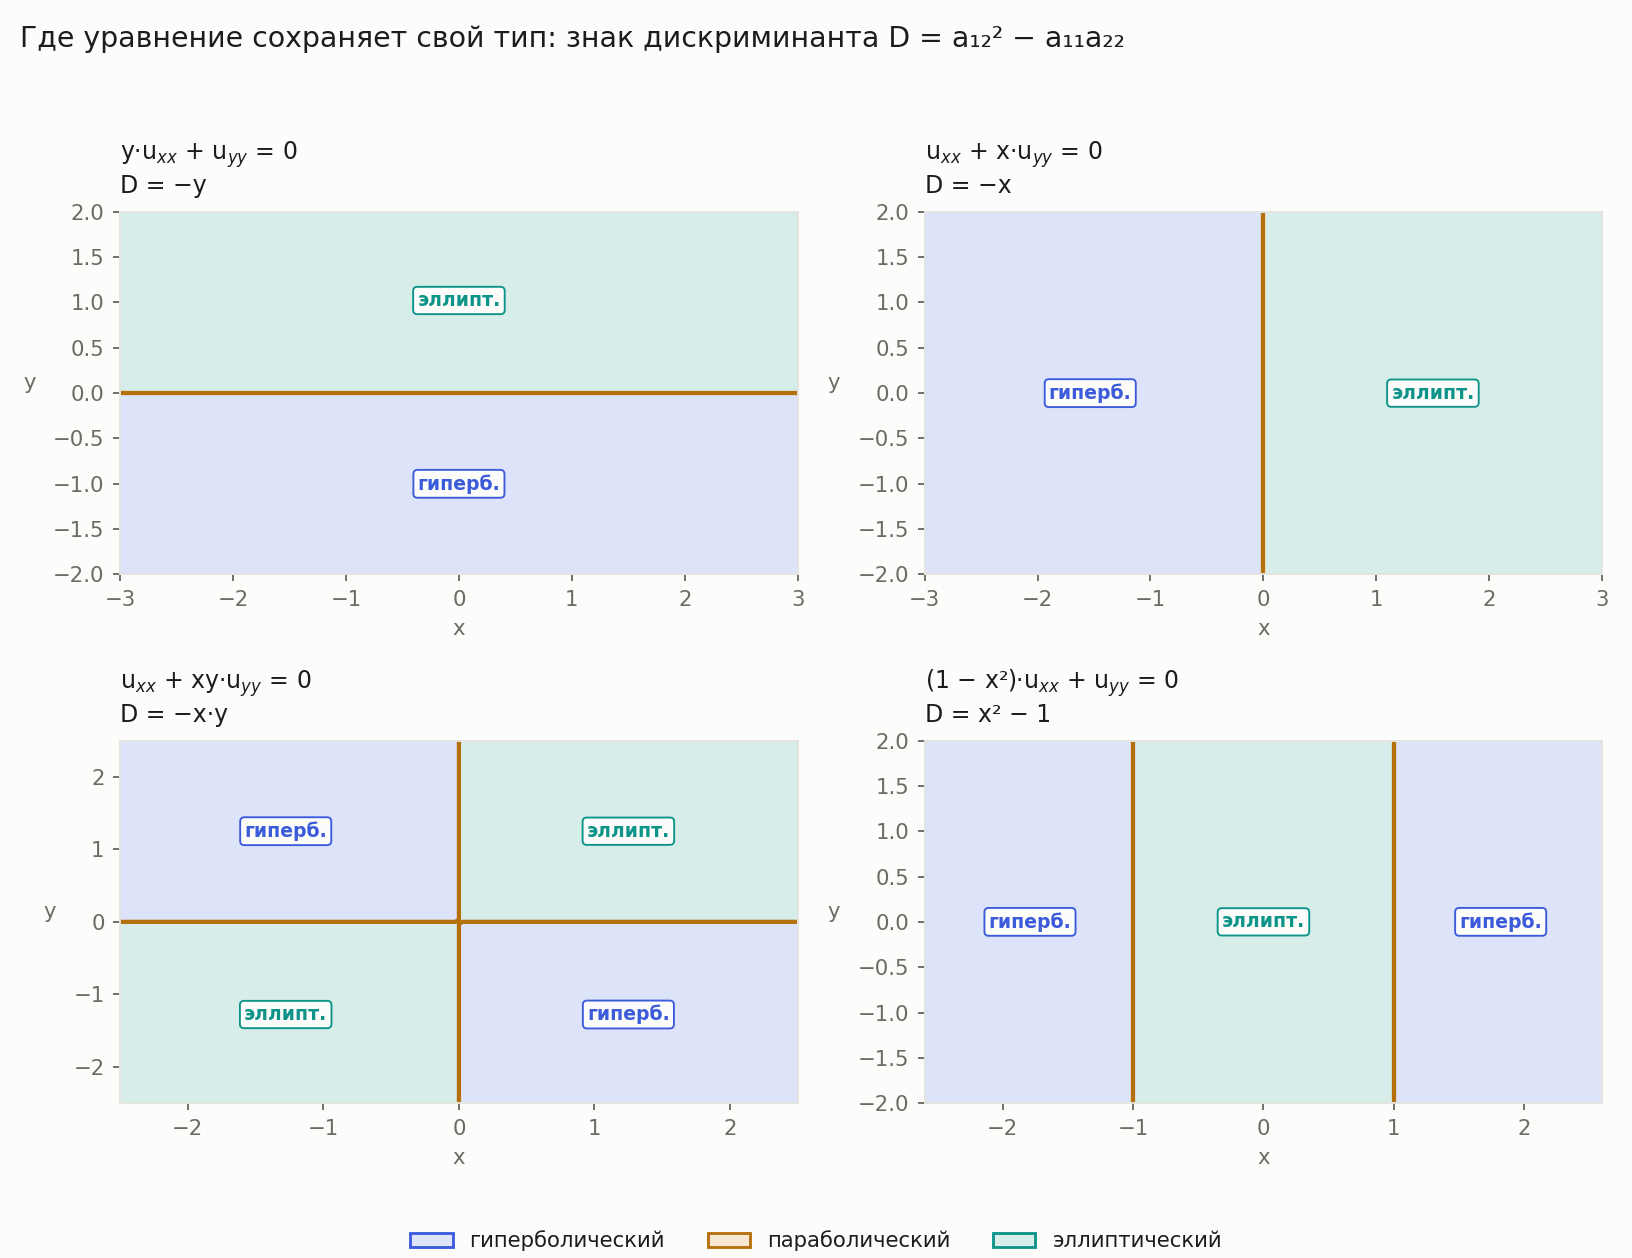
\includegraphics[width=\textwidth]{figures/regions_gallery.png}
\caption{Карты областей сохранения типа}
\label{fig:gallery}
\end{figure}

% ======================================================================
\section{Тестирование}

Для проверки программы разработан набор из 96 автоматических тестов
(модуль \texttt{unittest}); все тесты выполняются успешно. Эталонные значения
взяты из лекции и разбора примеров к ней. Проверяются:
\begin{itemize}
  \item обращение матриц, в том числе с радикалами (матрица $C$ примера~1);
  \item совпадение $\beta$, $C$ и $P$ в примерах~1 и~2 с разбором к лекции;
  \item тождество $P^{\mathsf T}\!AP=\diag(\beta)$ для всех рассмотренных форм,
        включая форму без квадратов и вырожденные формы;
  \item типы и замены для классических уравнений, случай $a_{11}=0$;
  \item обращение в нуль нужных коэффициентов $\bar a_{11},\bar a_{12},\bar a_{22}$
        и условие $J\neq0$;
  \item области и замены для уравнения Трикоми и уравнений с $D=-x$, $D=-xy$;
  \item совпадение типа, найденного двумя методами (таблица~\ref{tab:agree}).
\end{itemize}

\begin{table}[H]
\centering\small
\renewcommand{\arraystretch}{1.25}
\caption{Сравнение метода Лагранжа и метода характеристик}
\label{tab:agree}
\begin{tabular}{@{}ccccc@{}}
\toprule
$(a_{11},a_{12},a_{22})$ & $\beta$ & Тип (метод Лагранжа) & $D$ & Тип (метод характеристик)\\
\midrule
$(1,0,-1)$       & $(1,-1)$ & гиперболический & $1$            & гиперболический\\
$(1,0,1)$        & $(1,1)$  & эллиптический   & $-1$           & эллиптический\\
$(1,0,0)$        & $(1,0)$  & параболический  & $0$            & параболический\\
$(1,1,5)$        & $(1,1)$  & эллиптический   & $-4$           & эллиптический\\
$(1,-1,1)$       & $(1,0)$  & параболический  & $0$            & параболический\\
$(0,\frac12,0)$  & $(1,-1)$ & гиперболический & $\frac14$      & гиперболический\\
$(2,3,1)$        & $(1,-1)$ & гиперболический & $7$            & гиперболический\\
$(-1,0,1)$       & $(-1,1)$ & гиперболический & $1$            & гиперболический\\
$(3,-2,4)$       & $(1,1)$  & эллиптический   & $-8$           & эллиптический\\
\bottomrule
\end{tabular}
\end{table}

% ======================================================================
\section*{Заключение}

Реализованы все три пункта задания. Для уравнений с постоянными коэффициентами тип
и замена переменных определяются двумя способами: методом Лагранжа для
произвольного числа переменных и методом характеристик для двух переменных;
результаты методов согласованы. Разработан интерактивный виджет, который
пересчитывает тип, замену переменных и канонический вид при изменении
коэффициентов. Для уравнений с переменными коэффициентами определяются области
сохранения типа и выполняется приведение к каноническому виду в каждой области.
Типы уравнений и замены переменных в разобранных примерах совпадают с
приведёнными в лекции.

\end{document}
